\documentclass{article}
\usepackage{graphicx} % Required for inserting images
\usepackage{tocloft}  % Required for customizing table of contents
\usepackage{ulem} % Pakiet do przekreślania tekstu
\usepackage[T1]{fontenc} % Pakiet do polskich znaków
\usepackage[utf8]{inputenc} % Pakiet do polskich znaków
\usepackage{booktabs} % Pakiet do tabel
\usepackage[table,xcdraw]{xcolor} % Pakiet do kolorowania tabel
\usepackage{hyperref} % Pakiet do linków
\usepackage{graphicx} % Pakiet do obrazów
\graphicspath{ {/home/kamil/Downloads} } % Ścieżka do obrazów
\usepackage{float} % Pakiet do obrazów


\title{Homework-System-Decision-Methods}
\author{Kamil Badowicz}
\date{February 2024}

% Redefine the \cftsecleader command to add dots between page numbers and section names
\renewcommand{\cftsecleader}{\cftdotfill{\cftdotsep}}

\begin{document}

\maketitle

\tableofcontents

\section{Section}
\subsection{Subsection}
\subsubsection{subsubsection}

\cite{ref1}~Aleksy Fedorowicz Karamazow był trzecim synem właściciela ziemskiego, Fedora Pawłowicza Karamazowa, którego tragiczna i tajemnicza śmierć narobiła w swoim czasie wiele hałasu.
Ziemianin ów jak go powszechnie nazywano, mimo, że całe prawie życie spędził poza obrębem swych ziemskich posiadłości był to szczególny, jakkolwiek dość często zdarzający się typ człowieka. Obok lichego charakteru i rozpustnych skłonności, zdawał się być zupełnie pozbawiony zdrowego rozsądku, był, jak to mówią, „narwany”, z tych jednak narwanych, którzy umieją wybornie prowadzić własne interesa majątkowe, ale też tylko te. I tak naprzykład, rozpocząwszy od bardzo małego, jako właściciel drobnego kawałka ziemi, prowadził życie hulaszcze, żywiąc się przytem przeważnie po cudzych domach, a w chwili śmierci znaleziono przy nim przeszło sto tysięcy gotówki. Z tem wszystkiem słynął on w okolicy, jako zupełnie zwaryowany półgłówek, trzeba tu jednak dodać, że większej części swych szaleństw dokonał niezmiernie rozumnie i chytrze, a narwanie jego miało pewne specyalne, czysto narodowe cechy. Fedor Pawłowicz był dwa razy żonaty. Z pierwszego małżeństwa miał jednego syna, Dymitra, z drugiego dwóch: Iwana i Aleksego. Pierwsza jego żona pochodziła z zamożnej i bardzo znanej w okolicy szlacheckiej rodziny Mjusowów, którzy posiadali znaczne dobra. Jakim sposobem dziewczyna posażna, piękna, a przytem, jak na owe czasy, niepospolicie wykształcona, mogła wyjść za mąż za takiego marnego półgłówka, jakim był Karamazow, tego nie silę się wyjaśnić. Sam jednak znałem pannę z przeszłego „romantycznego” pokolenia, która żywiła przez lat kilka zagadkową miłość do pewnego jegomościa, za którego zresztą wyjść mogła każdej chwili najspokojniej w świecie. Mimo to, potrafiła sobie znaleźć tysiące urojonych przeszkód i przeciwności, które zniewoliły ją do rzucenia się ze szczytu stromej i wysokiej skały w głąb bystrej i głębokiej rzeki, gdzie też istotnie utonęła, jedynie tylko dlatego, aby się stać podobną do szekspirowskiej Ofelji. I to tak dalece, że gdyby w tem miejscu zamiast pięknej, malowniczej i wysokiej skały znajdował się zwykły, płaski, prozaiczny brzeg, samobójstwo to nie nastąpiłoby z pewnością. Fakt to jest autentyczny, a nie należy zapominać, że zaszło u nas niemało podobnych w ciągu trzech ostatnich pokoleń. Postępek Adelaidy Mjusow należał do tejże kategoryi zjawisk, a popełniła go niezawodnie pod wpływem owych nieuchwytnych, obcych wpływów i rozprzężenia myśli.

\subsubsection[Short title here]{Longer title here}

Czy chciała w ten sposób zaznaczyć kobiecą swą samodzielność, idąc wbrew panującym przesądom i despotycznym zachciankom rodziny? Czy usłużna wyobraźnia zrobiła w jej oczach Fedora Pawłowicza śmiałym szydercą i dzielnym szermierzem tej nowej, prowadzącej do wszelkiego dobra epoki? podczas gdy był to tylko lichy pajac, podszyty pieczeniarzem. Dość, że została jego żoną; a co było najciekawsze, że musiał ją Fedor Pawłowicz wykraść, czem ją najmocniej zadowolnił.
Fedor Karamazow, którego stanowisko towarzyskie było jeszcze wówczas bardzo skromne, gotów był na wszelkie kawały, byleby zrobić karyerę. Spokrewnienie się z arystokratyczną rodziną, a przytem zdobycie posagu, było, oczywiście, rzeczą bardzo dla niego nęcącą, co się tyczy jednak wzajemnej miłości, nie było jej prawdopodobnie z żadnej strony. Adelaida Iwanowna, mimo swej piękności, nie wzbudziła wcale głębszych namiętności w sercu swego męża, a był to jedyny wypadek w życiu tego człowieka, oddanego namiętnościom prawie wyłącznie miłosnym, który gonił ochoczo za każdą napotkaną spódniczką. Ta jedna tylko wśród wszystkich innych nie wywierała na niego żadnego wrażenia.
\subsection{Whateva}

Adelaida Iwanowna zdała sobie sprawę bardzo prędko po ślubie, że dla męża swego odczuwa tylko pogardę. Naturalnie, skutki tego wzajemnego stosunku dały się uczuć z błyskawiczną szybkością. Rodzina pani Karamazow dała się bardzo prędko przebłagać i oddała jej cały należny jej posag, mimo to, stosunki między małżonkami stały się bardzo burzliwe i rozpoczęły się nieustające sceny. Opowiadano, że w sporach tych młoda małżonka okazała daleko więcej godności i szlachetności, niż mąż, który, jak się później pokazało, wyłudził od niej odrazu cały jej kapitał, wynoszący 25,000 rubli, a następnie usiłował przejąć w posiadanie, za pomocą podrobionego aktu kupna, wioskę jej i dom w mieście, stanowiący jej spadek po rodzicach. Byłoby mu się to, zapewne, udało, dzięki, poprostu, uczuciu wstrętu i pogardy, jakie budził w swojej żonie, która zgodziłaby się na wszystko, byle się go módz pozbyć; na szczęście jednak, rodzina jej wdała się w to i powściągnęła jego chciwość. Opowiadano także, że przychodziło nawet do zniewagi czynnej, że jednak biła tu przedewszystkiem małżonka, dama odważna, prędka, gorącego temperamentu, a przytem obdarzona niepospolitą siłą fizyczną. W końcu Adelaida Iwanowna rzuciła dom i męża, i uciekła z ubogim nauczycielem seminaryum, pochodzącym z niższych warstw ludności, zostawiając synka Dymitra.
Natychmiast po jej wyjeździe, Karamazow zaprowadził u siebie rodzaj haremu, zapijając się przytem bez pamięci, w antraktach zaś jeździł po całej prawie okolicy, skarżąc się, ze łzami w oczach, na żonę każdemu, kto chciał tych skarg słuchać.
Przy tej sposobności opowiadał on o żonie swojej szczegóły, o jakich każdy inny mąż nie wspominałby nawet sam przed sobą bez uczucia wstydu. — W ogóle sprawiało mu, zda się, dziwną przyjemność odgrywać przed każdym śmieszną rolę zdradzonego męża, popisywał się prawie swoją krzywdą, to też żartownisie mówili mu. — „Wyglądacie, Fedorze Pawłowiczu, jakbyście dostąpili wyższej rangi, takie zadowolenie bije od was pomimo waszych strapień”. — Niektórzy utrzymywali, że Karamazow udaje tylko nieświadomość, zdając sobie wybornie sprawę ze śmiesznej strony swego położenia, któż jednak wiedzieć może, czy nie było w tem i rzeczywistej naiwności. — W końcu udało mu się natrafić na ślad zbiegłej swej małżonki. Biedaczka przebywała w Petersburgu wraz ze swym seminarzystą, i zaczynała właśnie puszczać się na pełne fale emancypacyi. — Fedor Pawłowicz zakłopotał się tem cokolwiek i zaczął nawet wybierać się do Petersburga, nie wiedząc właściwie, dlaczego? i poco? Możeby nawet rzeczywiście tam pojechał, gdyby nie to, że powziąwszy takie postanowienie, uczuł się w obowiązku dodać sobie animuszu przed drogą na swój zwykły sposób, t. j. oddając się bezprzykładnej pijatyce.
Tymczasem rodzina jego żony otrzymała wiadomość o jej śmierci. Umrzeć miała gdzieś na poddaszu z tyfusu. W chwili otrzymania tej wiadomości, Fedor Pawłowicz był zupełnie pijany. Opowiadano o nim, że wybiegł wówczas na ulicę z wzniesionemi do góry rękami, krzycząc na cały głos z radością: „Jestem wolny”. Inni utrzymywali, że płakał, jak małe dziecko, aż żal było patrzeć na niego, mimo wszystkich jego wad. — Bardzo być może, że jedno i drugie było prawdą. Cieszył się, prawdopodobnie, swojem oswobodzeniem i opłakiwał jednocześnie tę, która oswobodziła go swą śmiercią. — W znacznej ilości wypadków ludzie, nawet źli, znajdują więcej w sobie prostoduszności i dobroci, niżbyśmy mogli przypuszczać, a zauważyć to możemy i sami na sobie.



\subsubsection[short]{wololo}

Lorem ipsum dolor sit amet, consectetur adipiscing elit. Donec facilisis tellus ac tempor finibus. Sed placerat arcu ut urna blandit, at feugiat augue blandit. Nulla congue metus a odio luctus, eu finibus erat tempus. Integer porttitor mi ac velit iaculis, ut aliquam turpis bibendum. Praesent

\section{Style tekstów}

\subsection{Pogrubienie}
\textbf{Lorem ipsum dolor sit amet}
\subsection{Kursywa}
\textit{Lorem ipsum dolor sit amet}
\subsection{Podkreślenie}
\underline{Lorem ipsum dolor sit amet}
\subsection{Rozmiar czcionki}
{\tiny Lorem ipsum dolor sit amet}
{\scriptsize Lorem ipsum dolor sit amet}
{\footnotesize Lorem ipsum dolor sit amet}
{\small Lorem ipsum dolor sit amet}
{\normalsize Lorem ipsum dolor sit amet}
{\large Lorem ipsum dolor sit amet}
{\Large Lorem ipsum dolor sit amet}
{\LARGE Lorem ipsum dolor sit amet}
{\huge Lorem ipsum dolor sit amet}
{\Huge Lorem ipsum dolor sit amet}
\subsection{Przekreślenie}
\sout{Lorem ipsum dolor sit amet}
\newline
\textbf{\underline{\textit{\sout{{\LARGE Different size, underlined, cursive, bolded and sout}}}}}
\section{Środowiska}
\subsection{Listy}
\subsection{Równania}
\subsection{Tabele}
\subsection{Obrazy}


\section{Środowiska}
\subsection{Listy}
\paragraph{Unordered list}
\begin{itemize}
    \item Unordered list item 1
    \item Unordered list item 2
    \item Unordered list item 3
 \end{itemize}
 
 \paragraph{Ordered list}
 \begin{enumerate}
    \item Ordered list item 1
    \item Ordered list item 2
    \item Ordered list item 3
 \end{enumerate}
 
\subsection{Równania}
\paragraph{Inline equation}: 
Wzór na deltę jest równy $b^2-4ac$.

\paragraph{Display equation}:
\[
x_1 = \frac{-b + \sqrt{b^2 - 4ac}}{2a}
\]

\[
x_2 = \frac{-b - \sqrt{b^2 - 4ac}}{2a}
\]



\subsection{Tabele}

Tutaj bedzie tabela

\begin{center}
    \begin{table}[H]
        \centering
        \begin{tabular}{lcr}
        \toprule
        Ordinal no                   & \multicolumn{1}{l|}{Model Description}    & Results (\%)                          \\ \midrule
        \cellcolor[HTML]{9AFF99}left & {\color[HTML]{986536} centered}           & \cellcolor[HTML]{CBCEFB}right         \\ \midrule
        \textbf{left}                & \cellcolor[HTML]{FFFE65}\textbf{centered} & {\color[HTML]{6200C9} \textbf{right}} \\ \bottomrule
        \end{tabular}
    \end{table}
    Table 1 - Example of a table with different cell colors and text colors
    Table generated using \href{https://www.tablesgenerator.com/}{Table Generator}
\end{center}

The universe is immense and it seems to be homogeneous, in a large scale, everywhere we look at.


\begin{center}
    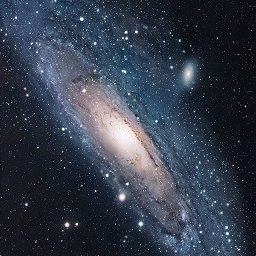
\includegraphics{galaxy.jpg}
\end{center}
\begin{center}
    \textbf{Figure 1} - A galaxy
\end{center}

\begin{thebibliography}{9}
\bibitem{ref1} Fiodor Dostojewski, Bracia Kazamow, 1913, \url{https://pl.wikisource.org/wiki/Bracia_Karamazow/Rozdzia%C5%82_pierwszy/I}

\end{thebibliography}

\end{document}


